% Change to use the correct class file for your paper.
\documentclass{sig-alternate-10pt}

%\pagenumbering{arabic}

\usepackage{amsfonts}     % Adds math fonts, commands such as \begin{align}
\usepackage{array}        % Tables for use in math mode
\usepackage{booktabs}     % Elegant table-formatting library
\usepackage{bold-extra}   % Provides bf+sc (only in textbf+textsc env.)
\usepackage{bytefield}    % Formatting and layout of packets / bytefields
\usepackage[skip=5pt]{caption}
\usepackage{color}        % Allow the use and definition of colors
\usepackage{colortbl}     % Color table cells
\usepackage{comment}      % Provides \begin,\end{comment} for large blocks
\usepackage{cprotect}     % Allows verbatim, other formatting in macro args
\usepackage{endnotes}     % Footnotes pushed to the end of a document
\usepackage{gensymb}      % Adds useful symbols w/out math mode, e.g. \degree
\usepackage{graphicx}     % For importing graphics
\usepackage{epsfig}
\usepackage{hyperref}     % Creates hyperlinks from ref/cite 
\hypersetup{pdfstartview=FitH}
\usepackage{listings}     % in-line source code (poorly, consider minted)
\usepackage{mathtools}    % amsmath extension, adds more math formatting
\usepackage{multirow}     % Multiple row spacing in tables
\usepackage{nth}          % Typeset 33rd correctly as \nth{33}
%\usepackage[section]{placeins} % Don't let figs escape their sections
\usepackage{rotating}     % Rotates any object, note sideways != sidewaysfigure
%\usepackage[all=normal]{savetrees} % For when space is tight, read manual and
                          % selectively enable things. CAN BREAK CONF STYLES!!
\usepackage{soul}         % Provides \hl{} for highlighting
%\usepackage{subfig}
%\usepackage{subfigure}    % Complicated figure creation
\usepackage{subcaption}   % Replaces both subfig and subfigure
\usepackage[nofancy]{svninfo} % svn information in docs (req. svn:keywords)
\usepackage{tabularx}     % Complicated table creation
\usepackage{threeparttable} % Add footnotes to a table
\usepackage{units}        % For nice fractions, \nicefrac{1}{2} --> 1/2
\usepackage{url}          % Pretty printing of hyperlinks
\usepackage{xspace}       % Intelligently add spaces after commands

%\DeclareCaptionType{copyrightbox}

\newlength\SUBSIZE

\renewcommand{\arraystretch}{1.2} % Space out rows in tables

%\setlength\paperheight {11in}
%\setlength\paperwidth {8.5in}

% Set the graphics path
\graphicspath{{../figs/}{../images/build/}}

% No space between bibliography items:
\let\oldthebibliography=\thebibliography
  \let\endoldthebibliography=\endthebibliography
  \renewenvironment{thebibliography}[1]{%
    \begin{oldthebibliography}{#1}%
      \setlength{\parskip}{0ex}%
      \setlength{\itemsep}{0ex}%
  }%
  {%
    \end{oldthebibliography}%
  }
\setlength{\parindent}{5mm}

\begin{document}

\title{Stable Data from Simultaneous Networks}

% AUTHOR STYLE 1
\author{
 \alignauthor{John Scheible and Kevin Krakauer}\\
 \affaddr{Electrical Engineering and Computer Science Department}\\
 \affaddr{University of Michigan}\\
 \affaddr{Ann Arbor, MI 48109}\\
 \email{\{jrscheib,krakauer\}@umich.edu}
}

% AUTHOR STYLE 2
\begin{comment}
\author{
\begin{tabular}{cc}
  \multicolumn{2}{c}{Author 1$^\dagger$, Author 2$^\dagger$, Author 3$^\dagger$, Author 4$^\ddagger$, and Author 5$^\dagger$\vspace{0.3cm}} \\
  \affaddr{$^\dagger$Computer Science \& Engineering Division} & \affaddr{$^\ddagger$Electrical and Computer Engineering Dept} \\ 
  \affaddr{University of Michigan} & \affaddr{Diff School}\\
  \affaddr{Ann Arbor, MI 48109} & \affaddr{Diff Address}\\
  \affaddr{\{u1,u2,u3,u4\}@eecs.umich.edu} & \affaddr{diffemail@email.com} \\
\end{tabular}
}
\end{comment}

\conferenceinfo{EECS 582 -- Winter'13} {Jan 10--Apr 23, 2013, Ann Arbor, Michigan, USA.}
\CopyrightYear{2013}
\crdata{XXX-X-XXXXX-XXX-X}

\maketitle

\begin{abstract}
% ABSTRACT

In today's world, users and applications rely on omnipresent internet connectivity. Entire products and software systems are built upon the assumption that users are always connected to the internet. However, mobile devices with cellular data and WiFi capabilities often drop connectivity to navigate between available connections. This makes many ``always-connected" appliations less useful or completely useless. In this paper we present a set of policies that mitigate connection issues casued by simultaneous internet connection options. We believe that these policies can greatly increase the connectivity of mobile devices and more fully realize the always-connected environment many applications and users rely on every day.
\end{abstract}


\category{}{COM\-PU\-TER-COM\-MU\-NI\-CA\-TION NET-\\WORKS}{Mobile Communications}
\terms{Design, Experimentation, Measurement, Performance}
\keywords{Mobile phones, Connectivity, Uptime, Always-connected Always-on}

\newpage

% page limit          % 14.0 pg
% abstract            %  0.5 pg
\vfill\eject
\section{Introduction}
\label{sec:intro}

In the era of always-connected mobile devices, a new breed of application has arisen that depends on a constant connection between mobile devices and the Internet. Users have come to rely heavily on the always-connected property of these applications for regular and time-sensitive information. Applications that utilize always-on connections generally fall into these categories:

\begin{description}
\item[Notification-based] Applications relying on ``push notifications" to alert users to pertinent, time-sensitive information. This class of applications includes email clients alerting users to a new email, social applications (e.g. Facebook, social games) updating users on relevant events, messaging applications (e.g. iMessage, KaokaoTalk), applications capable of providing emergency alerts, and other services that must present information as it becomes available.
\item[Streaming] Applications streaming data that rely on constant Internet connectivity to deliver uninterrupted content. Common types of streaming applications include audio streaming (e.g. Pandora, Spotify), video streaming (e.g. Youtube, Netflix), and real-time multiplayer games. Voice-over-IP (VOIP) services are also becoming more common on mobile devices (e.g. Skype, KaokaoTalk). Major network operators currently have plans to transition their entire networks to ``IP-only" \cite{ATT:2012} moving all voice and messaging services to connectivity-reliant applications.
\end{description}

Always-connected applications require guarantees of Internet connectivity. These applications do not function correctly when they suffer from intermittent or prolonged downtime.

Notification-based applications can likely tolerate a few seconds of downtime, although it is easy to imagine scenarios in which an application cannot tolerate downtimes on the order of minutes. For instance, having a conversation via instant messaging becomes difficult, and not very ``instant" when Internet connectivity is lost.

Streaming applications, however, cannot tolerate such downtime. \emph{Real-time} streaming applications such as VOIP that cannot buffer for more than a few seconds absolutely cannot tolerate it. VOIP is impractical when the connection is dropped for more than a few seconds at a time. Applications that can buffer data, such as streaming video and audio applications, can tolerate some downtime, although in many cases this is limited to a number of seconds.

For these and other reasons, mobile devices aim to provide 100\% Internet connectivity uptime. Connections are either established over a cellular data network, such as GSM or LTE, or a WiFi connection. The general policy for choosing which connection to use is simple: always prefer usable WiFi connections over cellular data [TODO - cite]. This policy is presumably based on a set of assumptions:

\begin{itemize}
\item WiFi connections are always faster than cellular connections.
\item Stable WiFi connections are more reliable than stable cellular connections.
\item Customers are charged for their cellular connections by the amount of data used.
\end{itemize}

While these may have been true at one time, they are becoming less and less so every day. With the advent of widely-available technologies like 4G LTE, the gap between WiFi and cellular connection speed has been shrinking \cite{Huang:2012:CEP:2307636.2307658}. While data caps are a legitimate concern, if no data is preferable to mobile data, modern smartphone operating systems include the option to disable it. Therefore, these priorities should no longer be the only factors in choosing whether to connect to the Internet via WiFi or a cellular data network.

The ``WiFi first and always" policy creates serious problems for always-connected applications. In many everyday scenarios, Internet connectivity is lost while mobile devices cling to unusable or weak WiFi networks. In these scenarios, Internet connectivity could be maintained by utilizing a cellular data connection, but the device instead loses connectivity because it tries to connect to an unusable WiFi network.

Three specific instances of this problem stand out, as they affect the average mobile device user (this paper's authors included) by regularly disconnecting the device from the Internet when a cellular connection could be used:

\begin{enumerate}
\item The mobile device connects to a WiFi network that is too weak to send data over.
\item The mobile device connects to a WiFi network that requires authentication before the Internet can be accessed.
\item The mobile device remains connected to a WiFi network after the network becomes too weak to send data over.
\end{enumerate}

In all of these cases, mobile devices running the Android or iOS operating systems will often remain disconnected from the Internet until the user manually intervenes by forcing the device to abandon WiFi (usually by disabling the device's WiFi feature entirely). These problems can result in downtime anywhere between less than a second to as long as it takes for a user to recognize and resolve the issue affecting the mobile device. In each of these scenarios, Internet connectivity could be maintained by utilizing the cellular connection. The policies we propose to resolve these problems are:

\begin{description}
\item[Internet Access Testing] In order to address problems 1 and 2, we propose to test and judge the usability of WiFi networks before making decisions about whether to connect to them. The goal of this policy is to make informed decisions about whether connecting to a WiFi network can be done seamlessly (i.e. while maintaining connectivity) or whether it will result in loss of Internet connectivity.
\item[Predictive WiFi Abandonment] In order to address problem 3, we propose to periodically sample the strength of the WiFi network the mobile device is currently connected to. Using this data, we can predict whether a WiFi connection will become too weak to function, and switch to a cellular data connection before Internet connectivity is lost.
\end{description}

         % 1.5 pg
\section{Related Work}
\label{sec:related}

Most work in the area of smartphone network policies has been in the interest of moving traffic to WiFi \cite{Lee:2010:MDO:1921168.1921203}. This is presumably due to assumptions stated above and the belief that WiFi is superior to any mobile connection. WiFi connections are obviously favored, as Android will automatically connect to any recognized network it encounters \cite{Google:2013}. The fact that this problem exists is evidence that work done on WiFi connection decisions in smartphone operating systems has simply not considered the issues of pre-mature connection or delayed disconnection from WiFi.

In some sense we could consider efforts to improve mobile networks as working towards our same goal of constant connectivity. Increasing mobile network speed and reliability would reduce a user's reliance on less pervasive WiFi. The latest mobile standards such as LTE have been shown to be faster than home WiFi in some cases \cite{Huang:2012:CEP:2307636.2307658}. While great advances have been made, economic concerns still limit the amount of traffic reasonable to transfer over mobile networks\footnote{Visit any major Cell Network Carrier's website to the limits and rates they place on mobile data}, ruling out the possibility of eliminating the need for WiFi.       % 2.0 pg
%\clearpage
\section{Design}
\label{sec:design}

% SPECIFICALLY address each of the 3 problems presented in the intro. Show how one policy fixes 2 of the problems, and how the other fixes 1.

\subsection{Internet Access Testing} % TODO - ask John about this. I did a pretty small, crappy writeup
In order to address problems 1 and 2, we designed a policy that would ensure that a mobile device does not connect to a WiFi network until it knows it will be capable of reaching the Internet over said network. The test is simple: when a new WiFi network is encountered and the device is using cellular data, attempt to ping a well known website (in our case, umich.edu) via the new WiFi network. The test is repeated a certain number of times in order to ensure that the WiFi network is offering the mobile device a stable connection.

If the correct server responds to our GET request with a 200 response (indicating a successful request), the thread sleeps for a set amount of time (in our case, 3 seconds) and continues pinging until we hit the number of tests we want to conduct (in our case, 2).

If any of these tests fails, we terminate the WiFi connection, and continue to use the cellular connection. If all the tests succeed, the device is switched over to the WiFi network. This, optimally, will result in no connection downtime whatsoever, as the WiFi connection is not utilized until it has been tested for Internet accessibility.

The reason that access is tested multiple times over a time interval is to establish reasonable evidence that the connection will remain strong after testing is concluded. Were the connection only tested once, it is very easy to imagine that a connection which will only be reachable for a couple of seconds (i.e. a scenario where the device briefly skirts the network's periphery) could be deemed valid and thus connected to.

The system is activated whenever the device is utilizing its cellular data connection, and encounters a new WiFi network.\footnote{We did consider the possibility of testing each individual access point (rather than WiFi network) encountered, but this would result in a massive number of WiFi scans that would considerably drain the device's battery.}

\subsection{Predictive WiFi Abandonment}
In order to address problem 3, we designed a policy that would preemptively terminate connections that are likely to degrade to the point of unusability. Currently, a mobile Android device will not disconnect from a WiFi network until it knows that it cannot reach the network anymore. This leads to downtime while the device has not yet determined that reaching the network is impossible, but traffic is not reaching its destination. The idea of our policy is based on a simple concept: that such downtime can be prevented by predicting when the network will become unreachable, not when it already has become so.

The test itself monitors the strength of a device's current WiFi connection. This information is obtained by querying the device's WiFi radio, which returns a received signal strength indication (RSSI) value. The range of possible RSSI values varies greatly depending on the device in question (i.e. some devices return vales from 0 to 100, some return values from -200 to 0, etc.), and therefore each device must normalize the RSSI values in order to make decisions.

In order to predict when WiFi quality is degrading to the point that it is better to switch to cellular data than remain connected to WiFi, the device monitors the signal strength over time. When the signal strength drops below a certain threshold for a certain amount of time (on our device, -80 RSSI units for 6.9 seconds), the system disconnects from WiFi and switches to cellular data. Ideally, this switch will result in no outgoing packet loss, as outgoing traffic is immediately diverted from WiFi to the cellular data network.

The system is active whenever WiFi is being used, and runs as a background process.         % 3.0 pg
\section{Implementation}
\label{sec:impl}

We chose to implement and run our policies on a Samsung Galaxy Nexus running Android 4.2 Jelly Bean. The Galaxy Nexus is capable of connecting to 3G networks and came out it late 2011 and is widely used today.

Originally, we aimed to modify Android's source code in order to implement our policies. This would have given us a great degree of control over Android's WiFi decision making policies. However, Android's source is both poorly documented and poorly understood outside of its group of core developers as Google. Therefore, our best option became implementing our policies as an Android application running on top of the OS's preexisting WiFi management policies.

As we will discuss, this did create sub-optimal conditions for the policies. Because the application ran on top of Android's WiFi management code, we could not implement our policies in a completely ideal manner. We will make clear how this affected our implementation, and how we expected it to affect our evaluation.

The application itself allows users to select one of three policies: internet access testing (Bouncer), predictive WiFi abandonment (AbandonShip), and default Android WiFi policies. When the policy was selected, an Android broadcast receiver was registered [TODO - terminology?]. This broadcast receiver was activated whenever the state of the device's network connection changed (i.e. a WiFi connection was established). These receivers would activate the chosen policy when it became pertinent.

In order to evaluate how each of these policies affected Internet connectivity, the application sent UDP packets approximately every 100 milliseconds to a server on the Internet. This allowed us to gather data about when WiFi connections were usable and providing reliable internet connectivity. [TODO - redundant with evaluation?]

\subsection{Internet Access Testing - Bouncer}
Our implementation of internet access testing, Bouncer, was written as a thread spawned by the broadcast receiver. The alternative was to run it as a service, Android's analogue to a background process; however, the thread has to be active only as long as network testing occurs (in our case, about 3 seconds). Therefore, we felt that running it as a service would be wasteful.

Optimally, we would have tested new networks as the device came into contact with them, joining one if and only if it passes all testing. However, because Bouncer was implemented as an application, not at the operating system level, we could not prevent the device from joining WiFi networks.

Our solution was to, as soon as the device joins a new WiFi network, test the network. If all tests are passed, the thread ends and the WiFi connection is left untouched. However, if a network fails the test, we boot the device of the network, forcing it to use the cellular data connection.

Were the policy optimally implemented, we would have expected no downtime, assuming a usable cellular data connection. All WiFi Internet access testing would occur without disconnecting from cellular data, while applications continue to use the cellular data connection. The switch would then be made if and only if all tests were passed by the WiFi network.

However, because of the limitations imposed upon us, we had to force the device to disconnect from unsuitable WiFi networks after Android had decided to switch them. This, we expected, would lead to downtime while the device was connected to an unsuitable network and as the device moved back from WiFi to cellular data [TODO - mention in evaluation!]. Again, were we to have greater access to Android's internals, we would be able to prevent utilization of the connection entirely until it had passed our tests. Because we could not prevent Android from connecting to unsuitable networks, we were forced to break the WiFi connection after it had been established, which would result in downtime when the network is unusable.

We would also optimally be able to reestablish the cellular data connection's Internet access, before swapping network traffic to the cellular data connection. This would, ideally, result in no downtime, as a connection would constantly be available over which traffic could be sent.

The tests themselves attempted to establish an HTTP connection to a well known web site (umich.edu). If the server responded with a 200 (HTTP OK) response, the thread would sleep for 3 seconds before running again. This was repeated twice. If a test failed, the connection was abandoned, and the device was forced to use its cellular data connection.

\subsection{Predictive WiFi Abandonment - AbandonShip}
Our implementation of predictive WiFi abandonment, AbandonShip, was written as an Android service spawned by the broadcast receiver. When a WiFi connection was established, it would begin monitoring the strength of the WiFi network's signal strength over time.

Given a certain strength threshold (-80 RSSI units) and time threshold (6.9 seconds), the service monitored signal strength in order to determine whether the signal had degraded below the strength threshold for a time equal to or greater than the time threshold.

This data was kept in a single variable: the count of consecutive signal strength readings below the strength threshold. Whenever the signal strength exceed the strength threshold, the count was reset to 0.

Because signal strength is sampled approximately every 100 milliseconds, the duration of signal strength below the strength threshold in seconds can be calculated by multiplying the sub-strength reading count by 0.1. For example, 42 consecutive packets below the strength threshold corresponds to $ 42 \cdot 0.1 = 4.2 $ seconds.

When the calculated time exceeds the time threshold, the system determines that the connection is becoming weaker, and will likely degrade past the point of usability. It then disconnects from the WiFi network, forcing the device to utilize its cellular data connection.

Like Bouncer, this implementation would have benefited from a lower-level implementation. However, the hindrance on AbandonShip is not as great. The only problem is that Android does not know to expect the disconnection from WiFi. The sudden disconnection ``surprises" it, and, as we will see in the evaluation, causes some downtime as Android switches to the cellular data network.

\section{Evaluation}
\label{sec:eval}

Our application, in addition to implementing our WiFi policies, would connect to a server and send a UDP packet every 100 milliseconds, stamped with a sequence number. To evaluate the performance our policies, we performed several experiments, with and without the appropriate policies enabled. For each experiment we inspected which packets were received to determine how many packets were dropped.

We present the setup and results from two experiments here. Each were inspired by the second and third problem situations presented. To test the Internet Access Testing policy, aproached a store with complimentary WiFi requireing authentication. For Predictive WiFi Abandonment, we left a WiFi network which was known to one of the authors to lost internet connectivity as a smartphone left [TODO: This is worded terribly][TODO: Better names for subsections...]

\subsection{Internet Access Testing - The Panera Test}
The problem of connecting to WiFi, without user intervention, that is unable to reach the internet is not cleanly measured. The impact of this issue varies on the users habits and the time spent within the network. To demonstrate this issue, as well as our solution we designed a realistic scenario to carry out. 

The experiment started across a parking lot, connected to AT\&T's HSPA network. We approached a store with public WiFi, which the phone would connect to once in range. Upon arriving at the door, we waited for 30 seconds and then attempted to access Google.com, waiting 10 seconds after successfully loading the page (including any delay from authentication).

\begin{figure}
	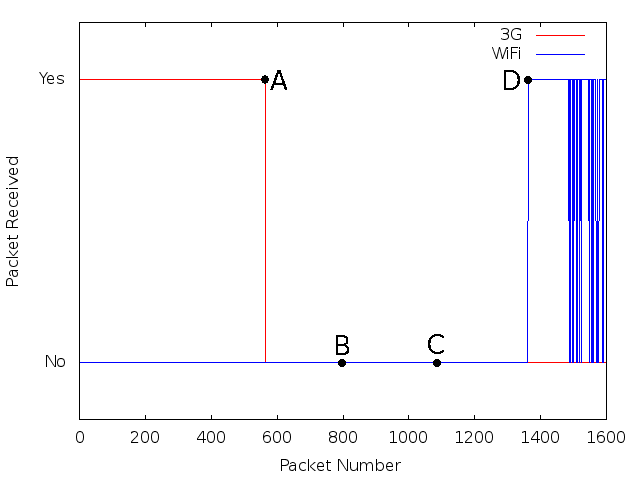
\includegraphics[width=0.5\textwidth]{paneraNoPolicy}
	\caption{TODO}
\end{figure}

Figure 2 shows, as expected, we did not receive a single packet from the time we walked within range of the WiFi to the time we attempted to access Google and accepted the store's terms and conditions. If a user left their phone in their pocket, rather than checking it as impulsively as the authors, they may never notice their phone had connected. In this case they wouldn't receive any incoming notifications until they left the store.

When run with Bouncer, the phone recieves a 302 HTTP code (a redirect to the store's terms and conditions page) after attempting to reach umich.edu. As per the implemented Bouncer policy, the phone then disconnects and reverts to the cell network. Figure 3 shows our drastically reduced downtime, present only because our implementation limits us from checking a WiFi network's Internet connection before the OS tears down the mobile connection.

\begin{figure}
	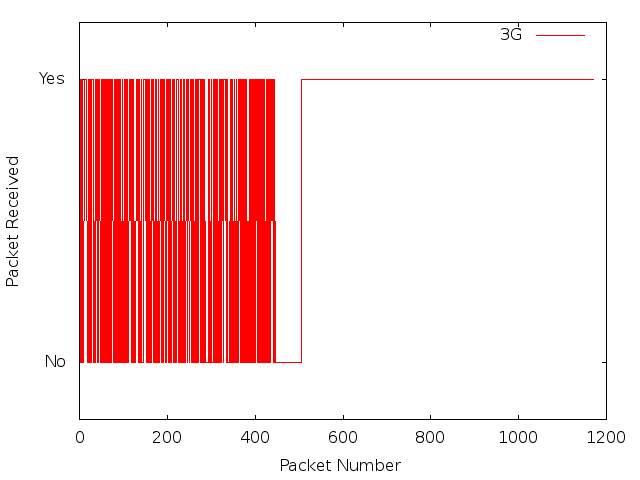
\includegraphics[width=0.5\textwidth]{paneraWithPolicy}
	\caption{TODO}
\end{figure}

\subsection{Predictive WiFi Abandonment - The Courtyards Test}
[TODO: Have Kevin check that this is a good description]
To evaluate our policy for disconnecting from poor WiFi connection, we began in a WiFi network which the authors had experienced disconnection issues from. From a starting position, connected to WiFi, we took a set route, leaving the range of the network. The route took us well out of the range of the access point, testing the transition from WiFi to cellular data.

The stock policy resulted in little to no connectivity at the perimeter of the network range. As seen in figure 4, a substantial number of packets are dropped before finally transitioning to the cellular connection. Another burst of packets are lost shortly after, when the phone tries to reconnect to the network it just left. This demonstrates a pattern the authors experienced which interrupts streaming content, and provides a generally poor user experience.

\begin{figure}
	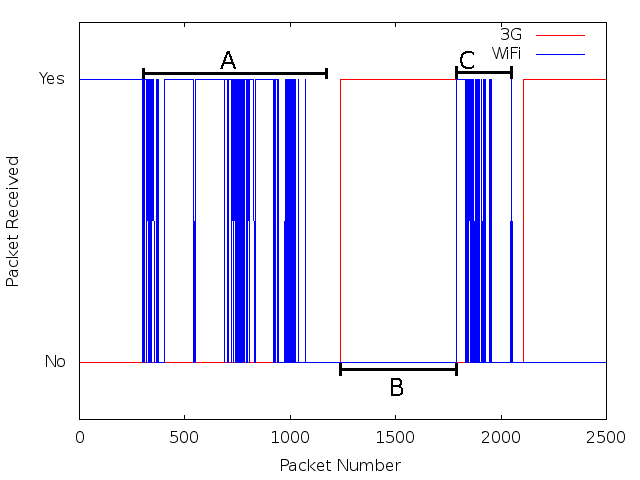
\includegraphics[width=0.5\textwidth]{leavingCourtyardsNoPolicy}
	\caption{TODO}
\end{figure}

When run with the Abandon Ship policy, as demonstrated by figure 5, the phone disconnects much more promptly from WiFi. It then stays on the cell network maintaining a stable connection. 

\begin{figure}
	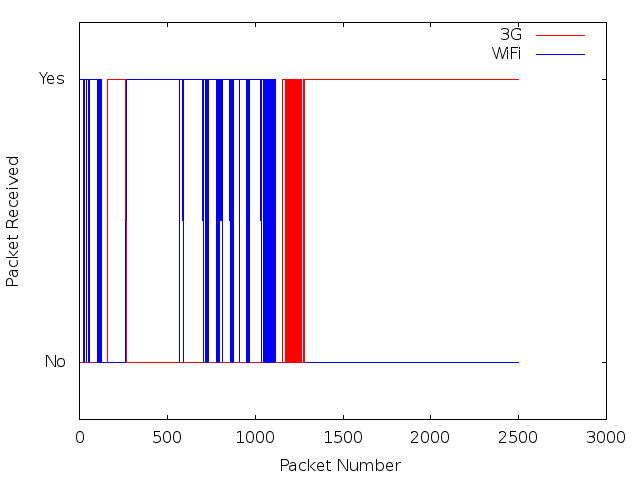
\includegraphics[width=0.5\textwidth]{leavingCourtyardsWithPolicy}
	\caption{TODO}
\end{figure}

%\begin{figure}
%	\includegraphics[width=0.5\textwidth]{}
%	\caption{TODO}
%\end{figure}          % 4.0 pg
\section{Discussion}
\label{sec:disc}


\subsection{Limitations}

Due to limited (and often nonexistant) documentation of the Android source code, we were forced to make some sacrifices. Optimally, we would have liked to modify Android's network management source directly. However, the lack of information provided by Google's Android team made writing a new application the best and most feasible option.

This somewhat limited our ability to fully control the mobile device's network management policies because our software ran concurrently with Android's built-in network management. Thus, while we were able to control connectivity, it was impossible to prevent Android from making its own decisions about network connectivity.

Therefore, in cases 1 and 2, our application could not \emph{prevent} connection to unsuitable WiFi networks. Instead, when such a connection occured, we detected the connection and terminated it as fast as Android's framework allows for. In case 3, Android's existing WiFi management policies did not interfere with our policies because we propose to drop connections \emph{before} Android acts.

Additionally, because we only worked with Android (as the other market leader, iOS, offers no control of WiFi/cell connection handling), it is possible that our data is specific to the domain of Android mobile devices. Other systems may have different WiFi/cell connection management policies.

Another limitation of our research is that 
          % 0.5 pg
\section{Conclusions}
\label{sec:conc}

Our policy implementations show that it is possible to increase connection uptime for mobile devices by clinging less strongly to WiFi networks. They allow devices to better support the always-connected environment that applications and users rely on every day in mobile computing.

It is important to note that the benefits of WiFi access testing and preemptive WiFi abandonment are demonstrable even with a suboptimal implementation. We strongly believe that the policies would show much better performance when implemented, ideally, as a part of Android's core operating system. The success of the policies as application-level implementations suggests that further investigation into integration into the Android operating system is worth pursuing.

Additionally, while we were unable to implement our policies on iOS devices, we observed that iOS suffered from all 3 of the issues addressed. Thus, we believe that the policies may also benefit iOS devices (as well as other mobile device operating systems such as Windows Phone 8).
          % 0.25 pg
\section{Acknowledgments}
\label{sec:ack}


           % 0.25 pg

%Uncomment this line if your paper has / uses end notes
%\theendnotes

{%\footnotesize
\raggedright
\bibliographystyle{abbrv}
\bibliography{bib}
}




\end{document}

